\documentclass[25pt, a0paper, portrait, margin=1cm, innermargin=0.5cm, colspace=1cm, subcolspace=0.5cm]{tikzposter}

\usepackage[utf8]{inputenc}
\usepackage[T1]{fontenc}
\usepackage{amsmath, amssymb, amsthm}
\usepackage{graphicx}
\usepackage{booktabs}
\usepackage{siunitx}
\usepackage{physics}
\usepackage[
  style=phys,
  backend=biber,
  articletitle=false,
  chaptertitle=false,
  pageranges=false,
  eprint=false,
  doi=false,
  url=false,
  maxbibnames=4,
  giveninits=true,
  uniquename=init,
]{biblatex}
\AtBeginBibliography{%
  \footnotesize
  \setlength{\bibitemsep}{0.25ex}%
  \setlength{\bibhang}{1.2em}%
}
\usepackage{caption}
\usepackage{hyperref}

\addbibresource{bibliography/references.bib}

% ---- Theme ----
\usetheme{Default}
\usecolorstyle{Default}

\makeatletter
% tikzposter wraps \title in \scalebox, which prevents line breaks
\def\title#1{\gdef\@title{#1}}
\renewcommand{\TP@maketitle}{%
  \noindent
  \begin{minipage}[c]{0.68\linewidth}
    \raggedright
    \color{titlefgcolor}%
    {\bfseries\Huge\scshape\@title\par}%
    \vspace*{0.8em}%
    {\Large\@author\par}%
    \vspace*{0.5em}%
    {\large\@institute}%
  \end{minipage}%
  \begin{minipage}[c]{0.30\linewidth}
    \centering
    
\includegraphics[height=6.5cm]{figures/units_logo.jpeg}\hspace{1.5em}%
    
\includegraphics[height=6.5cm]{figures/chirax_color.png}%
  \end{minipage}%
}
\makeatother

\title{Simulating Photoinduced Electron Dynamics for X-ray Absorption Spectroscopy and X-ray Natural Circular Dichroism in Molecules}
\author{\textbf{Manuel Fernando S\'anchez Alarc\'on}\textsuperscript{1,2}, Emanuele Coccia\textsuperscript{3}, and Majed Chergui\textsuperscript{2,4}}
\institute{\textsuperscript{1}Dipartimento di Fisica, University of Trieste, Italy \quad \textsuperscript{2}Elettra Sincrotrone, Trieste, Italy \quad \textsuperscript{3}Dipartimento di Scienze Chimiche e Farmaceutiche, University of Trieste, Italy \quad \textsuperscript{4}École Polytechnique Fédérale de Lausanne, Switzerland}

% ---- Block styling ----
\setlength{\parskip}{0.5em}

\begin{document}

\maketitle[width=774mm]

\begin{columns}
  \column{0.5}
  \block{Introduction}{
    Chirality is central to biochemistry and drug design~\cite{Chergui2016}.
    X-ray sources now extend chiroptical spectroscopy to core excitations, where resonant X-ray absorption (XAS) combines site specificity with strongly enhanced circular dichroism (XNCD)~\cite{Tanaka2005}.
    We address the need for theoretical assignments by propagating the time-dependent Schr\"odinger equation under an explicit pulse to compute XAS and XNCD in molecules with WaveT~\cite{Monti2023}, enabling interpretation of X-ray chiroptical spectra and ground- and valence excited-state pump--probe simulations~\cite{Sanchez2026}. 
  }

  \block{Methods}{
    \textbf{Real-time propagation (WaveT):}
    XAS and XNCD are obtained from the time-dependent Schr\"odinger equation in the length gauge or the velocity gauge~\cite{Pistillo2026}:
    \begin{equation}
      i\dv{}{t}\ket{\Psi(t)} = \qty(\hat{H}_0 + \hat{H}_I(t))\ket{\Psi(t)},
    \end{equation}
    where $\hat{H}_I(t)$ is the interaction Hamiltonian for the length gauge ($\hat{H}_I(t) = -\hat{\vec{\mu}}\cdot\vec{F}(t)$) or the velocity gauge ($\hat{H}_I(t) = \hat{\vec{p}}\cdot\vec{A}(t)$), and driven by a Gaussian-enveloped oscillatory pulse $\vec{F}(t) = \vec{F}_m \exp\!\left(-\frac{(t - t_0)^2}{2\sigma^2}\right)\sin(\omega_c t) = -\pdv{\vec{A}(t)}{t}$,
    with carrier frequency $\omega_c$, center $t_0$, width $\sigma$, and peak amplitude $\vec{F}_m$.

    \vspace{0.4em}
    \textbf{State-space expansion:}
    $\ket{\Psi(t)}$ is expanded in TDDFT eigenstates of $\hat{H}_0$.
    For ground-state (GS) spectra (core--valence separation, CVS):
    \begin{align}\label{eq:exp_core}
      \ket{\Psi(t)} = C_0(t)\ket{0} + \sum_{\lambda_c = 1}^{N_c}C_{\lambda_c}(t)\ket{\lambda_c}.
  \end{align}
    For excited-state (ES) spectra:
    \begin{align}\label{eq:exp_core_valence}
      \ket{\Psi(t)} = C_0(t)\ket{0} + \sum_{\lambda_c = 1}^{N_c}C_{\lambda_c}(t)\ket{\lambda_c} + \sum_{\lambda_v = 1}^{N_v}C_{\lambda_v}(t)\ket{\lambda_v}.
  \end{align}
    %Core and valence states are built in the 1h--1p (linear-response) manifold as linear combinations of singly excited Slater determinants.

    \vspace{0.4em}
    \textbf{Spectra (linear response):}
    With $\Delta\mu_q(t)=\mu_q(t)-\mu_q(0)$, $\Delta m_q(t)=m_q(t)-m_q(0)$ the time-dependent induced dipole moment and magnetic moment, along axis $q$, and $F_n^0(\omega)$ the Fourier transform of the field along axis $n$, the isotropic absorption and circular dichroism spectra are
    \begin{equation}
    \begin{gathered}
      P^A(\omega) = \frac{1}{3}\sum_{n \in \{x,y,z\}} P^A_{nn}(\omega),
      \quad
      P^{\mathrm{CD}}(\omega) = \frac{1}{3}\sum_{n \in \{x,y,z\}} P^{\mathrm{CD}}_{nn}(\omega), \\[0.4em]
      P^A_{nq}(\omega) = \frac{1}{2\pi F_n^0(\omega)}\int_0^\infty \Delta\mu_q(t)\,e^{i(\omega + i\Gamma)t}\,\dd t,
      \quad
      P^{\mathrm{CD}}_{nq}(\omega) = \frac{i}{2\pi \omega F_n^0(\omega)}\int_0^\infty \Delta m_q(t)\,e^{i(\omega + i\Gamma)t}\,\dd t,
    \end{gathered}
    \end{equation}
    where $\Gamma$ is a damping parameter (average excited-state lifetime).

    \vspace{0.4em}
    \textbf{Simulation pipeline:}

    \centering
    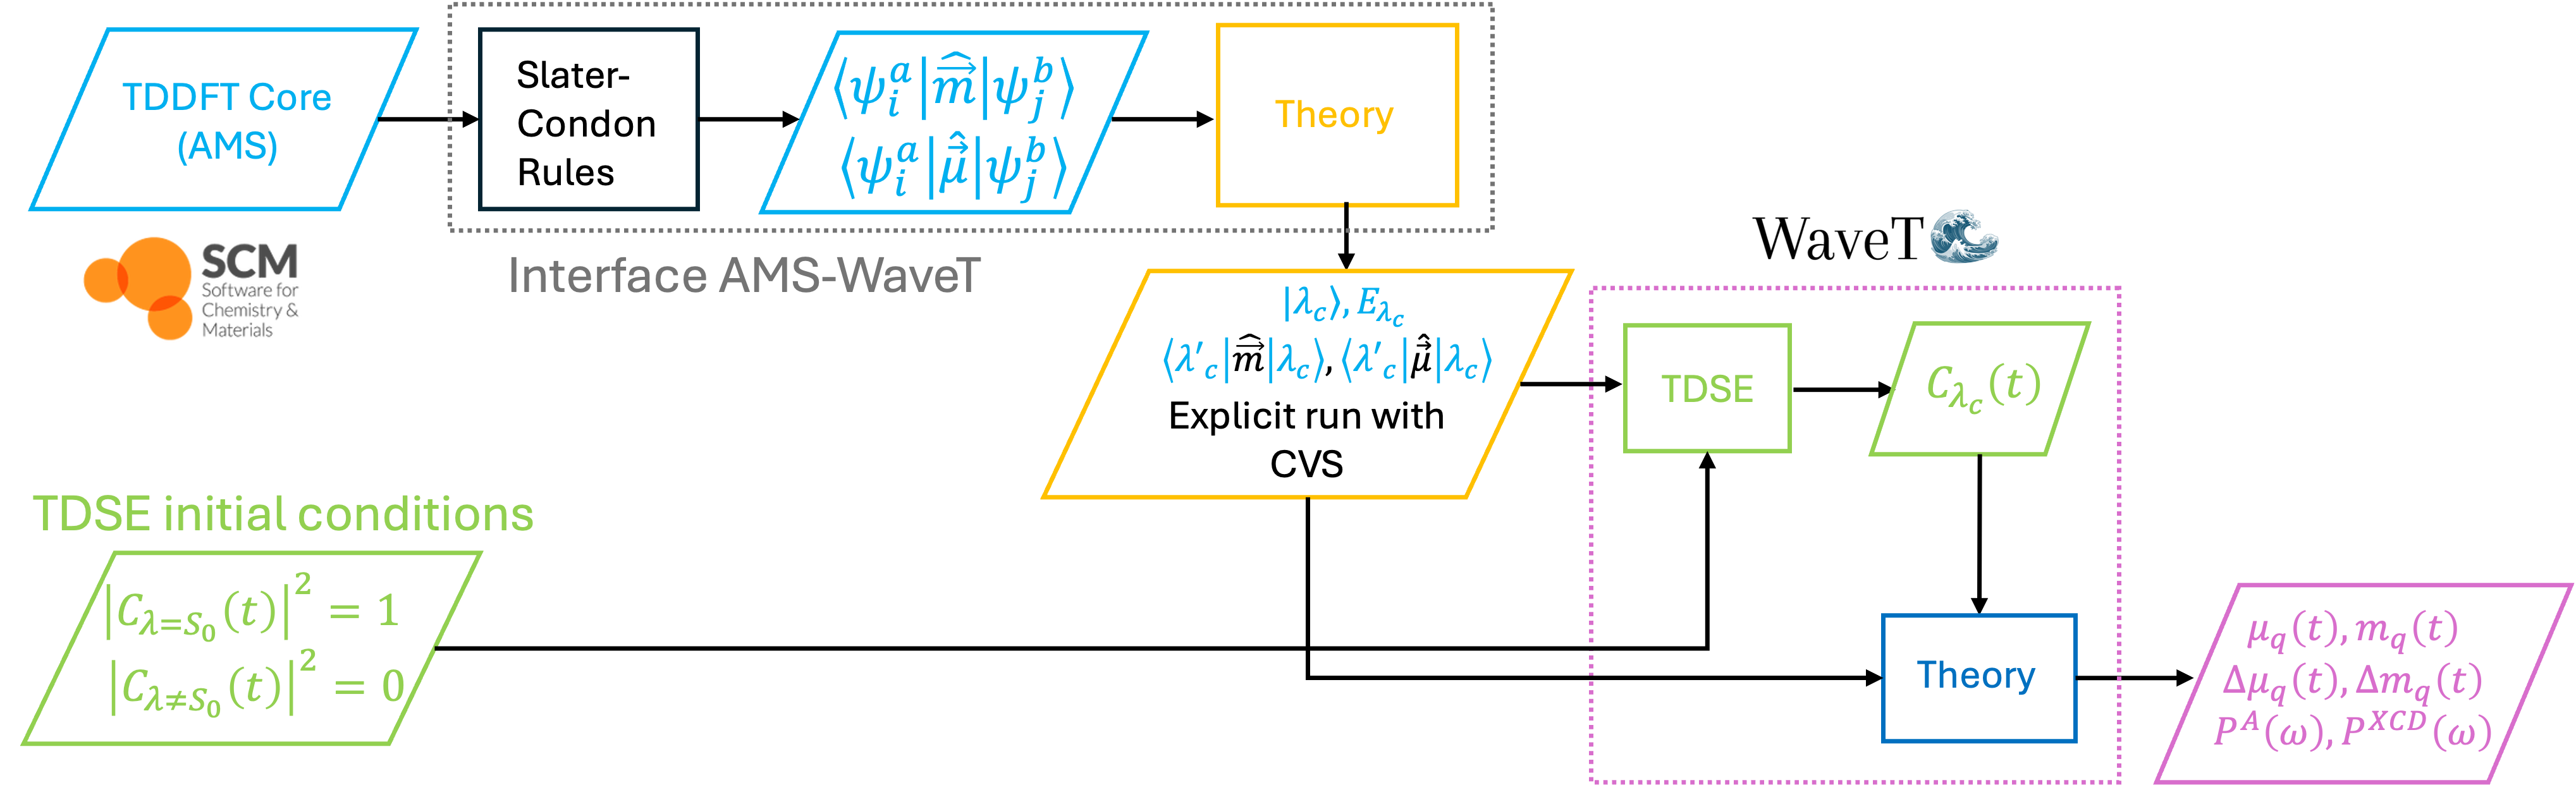
\includegraphics[width=0.8\linewidth]{figures/pipeline_gs.png}
    \captionof{figure}{Pipeline for the computation of ground-state XAS and XNCD in molecules.}
    \label{fig:pipeline_gs}
    \centering
    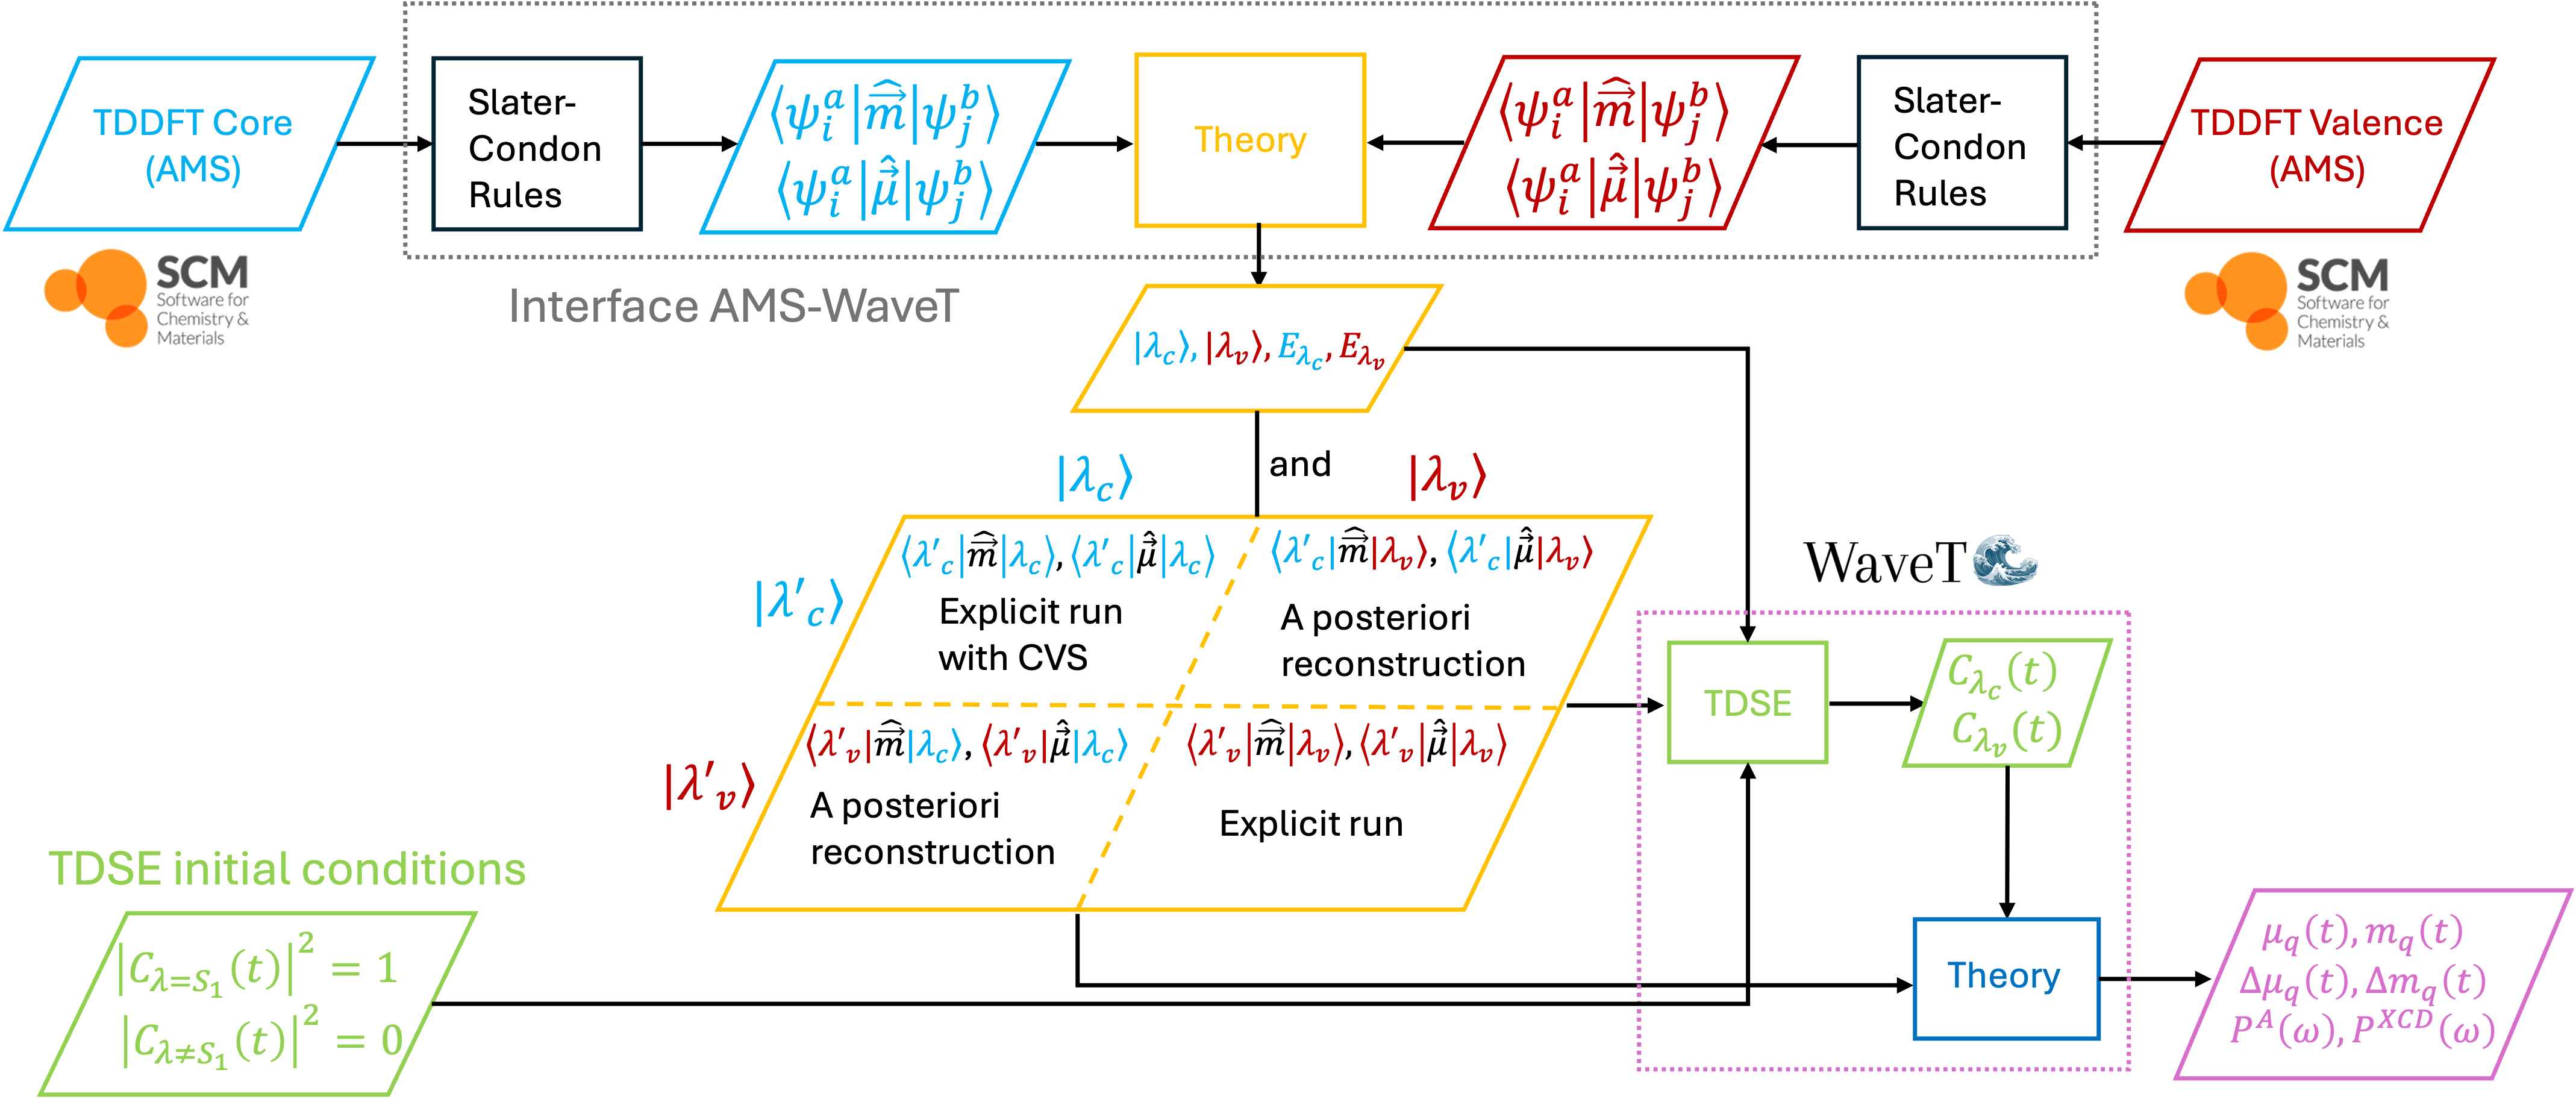
\includegraphics[width=0.8\linewidth]{figures/pipeline_es.png}
    \captionof{figure}{Pipeline for the computation of excited-state XAS and XNCD in molecules.}
    \label{fig:pipeline_es}  
  }

  \block{Acknowledgements}{
    We thank \dots for financial support.
  }

  \column{0.5}

  \block{Computational Details}{
    \textbf{System and theory:}
    (R)-methyloxirane; geometry from Andersen \textit{et al.}~\cite{Andersen2022} (reference for comparison).
    Ground state TDDFT simulations: DFT with ADF/AMS, CAM-B3LYP.

    \vspace{0.3em}
    \textbf{Basis sets (BS1--BS4):}
    C K-edge and valence results were benchmarked to choose an efficient, converged setup:
    BS1: C,O augmented TZP; H TZP.
    BS2: C QZP+1 diffuse; O,H TZP.
    BS3: C,O QZP+1 diffuse; H DZP.
    BS4: C,O QZP+1 diffuse; H TZP.

    \vspace{0.3em}
    \textbf{Core and valence states:}
    Core TDDFT under CVS (60 states retained).
    Valence TDDFT without orbital freezing (60 states retained).
    Real-time dynamics at the C K-edge: 17 core states and 60 valence states; core manifold limited to excitations below the C $1s$ ionization threshold.

    \vspace{0.3em}
    \textbf{Propagation:}
    97~fs trajectories with time step $\delta t = 0.12$~as, field intensity $I = 10^{4}$~W\,cm$^{-2}$, $\omega_c = 278$~eV (C K-edge XAS/XNCD), pulse FWHM 1~fs, $\tau = 1/\Gamma = 200$~a.u.
  }

  \block{Results and Discussion}{
    \noindent
    \begin{minipage}[t]{0.65\linewidth}
      \centering
      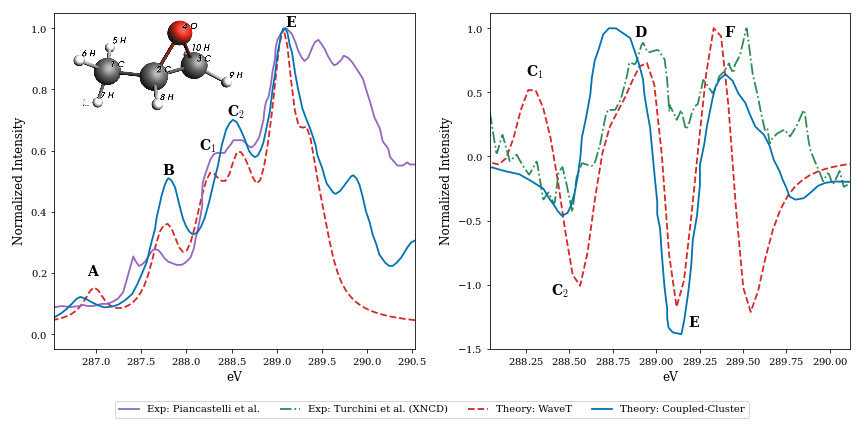
\includegraphics[width=\linewidth]{figures/xas_xcd_gs_codiff_lg_exp_cc.png}
      \captionsetup{width=\linewidth}
      \captionof{figure}{Experimental vs.\ computed ground-state XAS and XNCD for (R)-methyloxirane. Couple-Cluster data was obtained from Andersen \textit{et al.}~\cite{Andersen2022}, while experimental data was obtained from \cite{piancastelli2007,turchini2004}.}
      \label{fig:xas_xcd_gs_codiff_lg_exp_cc}

      \vspace{0.6em}
      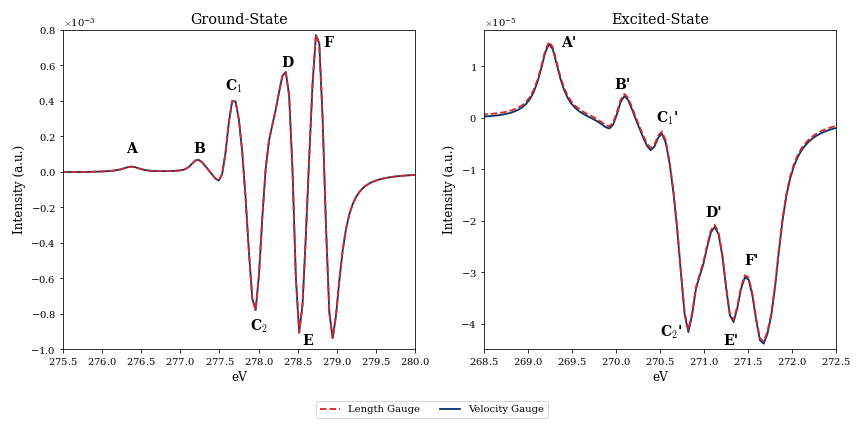
\includegraphics[width=\linewidth]{figures/xcd_gs_es_codiff_lg_vg.png}
      \captionof{figure}{Computed first-excited-state XNCD for (R)-methyloxirane.}
      \label{fig:xcd_gs_es_codiff_lg_vg}
    \end{minipage}%
    \hspace{0.03\linewidth}%
    \begin{minipage}[t]{0.25\linewidth}
      \centering
      \footnotesize
      \begin{tabular}{@{}lc@{}}
        \toprule
        Peak & Composition\\
        \midrule
        $A$ & \begin{tabular}{@{}r@{\quad}l@{}}
                71\%: & 1S (1C) $\rightarrow$ LUMO \\
                13\%: & 1S (1C) $\rightarrow$ LUMO \\
              \end{tabular} \\
        $B$ & \begin{tabular}{@{}r@{\quad}l@{}}
                34\%: & 1S (1C) $\rightarrow$ LUMO+3 \\
                30\%: & 1S (1C) $\rightarrow$ LUMO+1 \\
              \end{tabular} \\
        $C_1$ & \begin{tabular}{@{}r@{\quad}l@{}}
                26\%: & 1S (3C) $\rightarrow$ LUMO+3 \\
                25\%: & 1S (3C) $\rightarrow$ LUMO \\
              \end{tabular} \\
        $C_2$ & \begin{tabular}{@{}r@{\quad}l@{}}
                35\%: & 1S (3C) $\rightarrow$ LUMO \\
                19\%: & 1S (3C) $\rightarrow$ LUMO+1 \\
              \end{tabular} \\
        $D$ & \begin{tabular}{@{}r@{\quad}l@{}}
                35\%: & 1S (3C) $\rightarrow$ LUMO \\
                19\%: & 1S (3C) $\rightarrow$ LUMO+1 \\
              \end{tabular} \\
        $E$ & \begin{tabular}{@{}r@{\quad}l@{}}
                25\%: & 1S (2C) $\rightarrow$ LUMO+14 \\
                18\%: & 1S (2C) $\rightarrow$ LUMO+3 \\
              \end{tabular} \\
        $F$ & \begin{tabular}{@{}r@{\quad}l@{}}
                26\%: & 1S (2C) $\rightarrow$ LUMO+3 \\
                25\%: & 1S (2C) $\rightarrow$ LUMO+2 \\
              \end{tabular} \\
        \bottomrule
      \end{tabular}
      \captionsetup{width=\linewidth}
      \captionof{table}{Peak composition for ground-state XAS and XNCD.}
      \label{tab:xcd_peaks}
    \end{minipage}

    \centering
    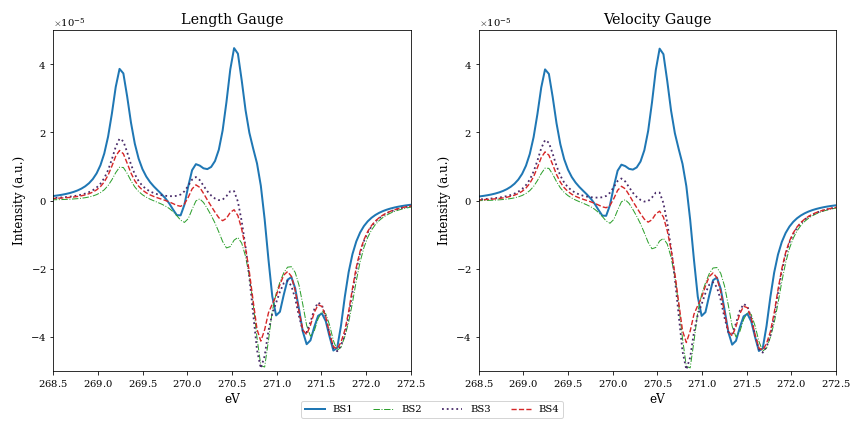
\includegraphics[width=0.57\linewidth]{figures/xcd_es_vcsame_lg_vg.png}
    \captionof{figure}{Basis set convergence of computed first-excited-state XNCD for carbon K-edge of (R)-methyloxirane. Core and valence calculations used to obtain the excited-state XNCD share the same basis set.}
    \label{fig:xcd_es_vcsame_lg_vg}
  }

  \block{Conclusions}{
    \begin{itemize}
      \item WaveT is a general framework for molecular XAS and XNCD, including excited-state spectra and prospective solvent effects (perturbative matrix method or COSMO).
      \item For (R)-methyloxirane, WaveT ground-state XAS and XNCD reproduce experiment and agree with coupled-cluster benchmarks.
      \item Ground- and excited-state core transitions are assigned unambiguously.
    \end{itemize}
  }

  \block{References}{
    \printbibliography[heading=none]
  }
\end{columns}

\end{document}
